\documentclass[
]{jss}

%% recommended packages
\usepackage{orcidlink,thumbpdf,lmodern}

\usepackage[utf8]{inputenc}

\author{
James Hollway\\Graduate Institute of\\
International and Development Studies \And Henrique Sposito\\Graduate
Institute of\\
International and Development Studies
}
\title{Working with Unspecified, Approximate, Uncertain, Sets and Ranges
of Dates with \pkg{messydates}}

\Plainauthor{James Hollway, Henrique Sposito}
\Plaintitle{Working with Unspecified, Approximate, Uncertain, Sets and
Ranges of Dates with messydates}
\Shorttitle{\pkg{messydates}: An R package for ISO's Extended Date/Time
Format}


\Abstract{
This paper presents the \pkg{messydates} package for R, which
facilitates working with `messy' dates. Messy dates are common when
studying historical and sometimes even current phenomena, and can create
various technical problems for the data analyst. The paper highlights
these problems and offers practical advice on how to solve them using
\pkg{messydates}. The paper also introduces a conceptual framework for
resolving messydates into more familiar date classes in R ready for
analysis.
}

\Keywords{dates, ISO, \proglang{R}}
\Plainkeywords{dates, ISO, R}

%% publication information
%% \Volume{50}
%% \Issue{9}
%% \Month{June}
%% \Year{2012}
%% \Submitdate{}
%% \Acceptdate{2012-06-04}

\Address{
    James Hollway\\
    Graduate Institute of\\
International and Development Studies\\
    Chemin Eugène-Rigot 2A\\
PO Box 1672\\
1211 Geneva 1\\
Switzerland\\
  E-mail: \email{james.hollway@graduateinstitute.ch}\\
  URL: \url{http://jameshollway.com}\\~\\
    }


% tightlist command for lists without linebreak
\providecommand{\tightlist}{%
  \setlength{\itemsep}{0pt}\setlength{\parskip}{0pt}}




\usepackage{amsmath}

\begin{document}



\hypertarget{introduction}{%
\section{Introduction}\label{introduction}}

Dates are often messy. Whether historical (or ancient), future, or even
recent, we often only know approximately when an event occurred, that it
happened within a particular period, an unreliable source means a date
should be flagged as uncertain, or sources offer multiple, competing
dates.

\pkg{messydates} implements for R the Extended Date/Time Format (EDTF)
annotations set by the International Organization for Standardization
(ISO) outlined in \href{https://www.iso.org/standard/70908.html}{ISO
8601-2\_2019(E)}. The standardised extended format allow for unambiguous
interpretation of dates and guarantee interoperability. These include
notation for:

\begin{itemize}
\tightlist
\item
  unspecified date( component)s, e.g.~\texttt{2012-XX-01} for the first
  of some unknown month in 2012 or \texttt{2012-01} for some unknown day
  in January 2012
\item
  approximate date( component)s,
  e.g.~\texttt{2012-01-12\textasciitilde{}} for approximately the 12th
  of January 2012
\item
  uncertain date( component)s, e.g.~\texttt{2012-01-12?} where this data
  point is based on an unreliable source
\item
  sets of dates, e.g.~\texttt{\{2012-01-01,2012-01-12\}} where the date
  can be either 1 January 2012 and 12 January 2012
\item
  ranges of dates, e.g.~\texttt{2012-01-01..2012-01-12} for all dates
  between the 1 January 2012 and 12 January 2012 inclusive
\end{itemize}

\pkg{messydates} contains a set of tools for constructing and coercing
into and from the \texttt{mdate} class. This date class allows regular
dates to be annotated to express unspecified date components,
approximate or uncertain date components, date ranges, and sets of
dates.

The package also includes a function for unpacking or expanding sets or
ranges of dates into all dates consistent with how the date or set of
dates is specified or annotated. Methods are also offered that can be
used to make explicit how researchers convert date imprecision into
precise dates for analysis, such as getting the \texttt{min()},
\texttt{max()}, or even a \texttt{random()} date from among the dates
consistent with a set or range of dates. This greatly facilitates
research transparency as well as robustness checks as we will
demonstrate below.

\hypertarget{motivation}{%
\subsection{Motivation}\label{motivation}}

As researchers, we often recognize this messiness but are required to
force non-existent precision on data so we can proceed with analysis.
For example, if we only know something happened in a given month or
year, we might just opt for the start of that month
(e.g.~\texttt{2021-07-01}) or year (\texttt{2021-01-01}), assuming that
to err on the earlier (or later) side is a justifiable bias. However,
this can create issues for inference in which sequence or timing is
important. The goal of \pkg{messydates} is to help with this problem by
retaining and working with various kinds of date imprecision.

\hypertarget{relationship-to-other-packages}{%
\subsection{Relationship to other
packages}\label{relationship-to-other-packages}}

\pkg{messydates} offers a new date class, but one that comes with
methods for converting from and into \texttt{base}, date classes such as
\texttt{Date}, \texttt{POSIXct}, and \texttt{POSIXlt}. It is thus fully
compatible with packages such as \pkg{lubridate}
\citep{grolemundDatesTimesMade2011} and \pkg{anytime}
\citep{eddelbuettelAnytimeEasierDate2019}. \pkg{messydates} is,
therefore, compatible (perhaps with an additional coercion step) with
all contemporary R packages for analysis.

\section[R code]{\proglang{R} code}\label{r-code}

\hypertarget{a-new-class}{%
\subsection{A new class}\label{a-new-class}}

\pkg{messydates} contains a set of tools for constructing and coercing
into and from the \texttt{mdate} class. This date class implements ISO
8601-2:2019(E) and allows regular dates to be annotated to express
unspecified date components, approximate or uncertain date components,
date ranges, and sets of dates. The function \texttt{as\_messydate()}
handles the coercion to \texttt{mdate} class.

\begin{CodeChunk}
\begin{CodeInput}
R> tibble::tribble(~Example, ~Date,
+                 "A normal date", as.character(Sys.Date()),
+                 "A future date", "2599-12-31",
+                 "A written date", "This is the first day of February, two thousand and twenty-one",
+                 "A historical date", "476",
+                 "An era date", "33 BC",
+                 "An approximate date", "2012-01-12~",
+                 "An uncertain date", "2001-01-01?",
+                 "An unspecified date", "2012-01",
+                 "A censored date", "..2012-01-12",
+                 "A range of dates", "2019-11-01:2020-01-01",
+                 "A set of dates", "2021-5-26, 2021-11-19, 2021-12-4") %>%
+   dplyr::mutate(base = as.Date(Date),
+                 lubridate = lubridate::as_date(Date),
+                 anytime = anytime::anydate(Date),
+                 messydates = messydates::as_messydate(Date))
\end{CodeInput}
\begin{CodeOutput}
# A tibble: 11 x 6
   Example             Date             base       lubridate  anytime    messy~1
   <chr>               <chr>            <date>     <date>     <date>     <mdate>
 1 A normal date       2022-09-06       2022-09-06 2022-09-06 2022-09-06 2022-0~
 2 A future date       2599-12-31       2599-12-31 2599-12-31 2599-12-31 2599-1~
 3 A written date      This is the fir~ NA         NA         NA         2021-0~
 4 A historical date   476              NA         NA         NA         0476  ~
 5 An era date         33 BC            NA         NA         NA         -0033 ~
 6 An approximate date 2012-01-12~      2012-01-12 2012-01-12 2012-01-12 2012-0~
 7 An uncertain date   2001-01-01?      2001-01-01 2001-01-01 2001-01-01 2001-0~
 8 An unspecified date 2012-01          NA         2020-12-01 2012-01-01 2012-0~
 9 A censored date     ..2012-01-12     NA         2012-01-12 NA         ..2012~
10 A range of dates    2019-11-01:2020~ 2019-11-01 2019-11-01 2019-11-01 2019-1~
11 A set of dates      2021-5-26, 2021~ 2021-05-26 NA         2021-05-26 {2021-~
# ... with abbreviated variable name 1: messydates
\end{CodeOutput}
\end{CodeChunk}

\hypertarget{annotate}{%
\subsection{Annotate}\label{annotate}}

Some datasets have, for example, an arbitrary cut off point for start
and end points, but these are often coded as precise dates when they are
not necessarily the real start or end dates. The annotate functions
helps annotate uncertainty and approximation to dates. Inaccurate start
or end dates can be represented by an affix indicating ``on or before'',
if used as a prefix (e.g.~\texttt{..1816-01-01}), or indicating ``on or
after'', if used as a suffix (e.g.~\texttt{2016-12-31..}). Approximate
dates are indicated by adding a \texttt{\textasciitilde{}} to year,
month, or day components, as well as groups of components or whole dates
to estimate values that are possibly correct
(e.g.~\texttt{2003-03-03\textasciitilde{}}). Day, month, or year,
uncertainty can be indicated by adding a \texttt{?} to a possibly
dubious date (e.g.~\texttt{1916-10-10?}) or date component
(e.g.~\texttt{1916-?10-10}).

\begin{CodeChunk}
\begin{CodeInput}
R> tibble::tibble(Beg = as_messydate(c("1816-01-01", "1916-01-01", "2016-01-01")),
+                End = as_messydate(c("1816-12-31", "1916-12-31", "2016-12-31"))) %>% 
+   dplyr::mutate(on_or_before = ifelse(Beg <= "1816-01-01", on_or_before(Beg), Beg),
+                 on_or_after = ifelse(End >= "2016-01-01", on_or_after(End), End),
+                 as_approximate = ifelse(End >= "2016-01-01", on_or_after(End), End),
+                 as_uncertain = ifelse(End == "1916-12-31", as_uncertain(End), End))
\end{CodeInput}
\begin{CodeOutput}
# A tibble: 3 x 6
  Beg        End        on_or_before on_or_after  as_approximate as_uncertain
  <mdate>    <mdate>    <chr>        <chr>        <chr>          <chr>       
1 1816-01-01 1816-12-31 ..1816-01-01 1816-12-31   1816-12-31     1816-12-31  
2 1916-01-01 1916-12-31 1916-01-01   1916-12-31   1916-12-31     1916-12-31? 
3 2016-01-01 2016-12-31 2016-01-01   2016-12-31.. 2016-12-31..   2016-12-31  
\end{CodeOutput}
\end{CodeChunk}

\hypertarget{expand}{%
\subsection{Expand}\label{expand}}

Expand functions transform date ranges, sets of dates, and unspecified
or approximate dates (annotated with `..', `\{ , \}', `XX' or
`\textasciitilde{}') into lists of dates. As these dates may refer to
several possible dates, the function ``opens'' these values to include
all the possible dates implied.

\begin{CodeChunk}
\begin{CodeInput}
R> dates_expand <- as_messydate(c("2001-01-01", "2001-01", "2001-01-01..2001-02-01",
+                                "{2001-01-01,2001-02-01}", "2001-XX-01"))
R> expand(dates_expand)
\end{CodeInput}
\begin{CodeOutput}
[[1]]
[1] "2001-01-01"

[[2]]
 [1] "2001-01-01" "2001-01-02" "2001-01-03" "2001-01-04" "2001-01-05"
 [6] "2001-01-06" "2001-01-07" "2001-01-08" "2001-01-09" "2001-01-10"
[11] "2001-01-11" "2001-01-12" "2001-01-13" "2001-01-14" "2001-01-15"
[16] "2001-01-16" "2001-01-17" "2001-01-18" "2001-01-19" "2001-01-20"
[21] "2001-01-21" "2001-01-22" "2001-01-23" "2001-01-24" "2001-01-25"
[26] "2001-01-26" "2001-01-27" "2001-01-28" "2001-01-29" "2001-01-30"
[31] "2001-01-31"

[[3]]
 [1] "2001-01-01" "2001-01-02" "2001-01-03" "2001-01-04" "2001-01-05"
 [6] "2001-01-06" "2001-01-07" "2001-01-08" "2001-01-09" "2001-01-10"
[11] "2001-01-11" "2001-01-12" "2001-01-13" "2001-01-14" "2001-01-15"
[16] "2001-01-16" "2001-01-17" "2001-01-18" "2001-01-19" "2001-01-20"
[21] "2001-01-21" "2001-01-22" "2001-01-23" "2001-01-24" "2001-01-25"
[26] "2001-01-26" "2001-01-27" "2001-01-28" "2001-01-29" "2001-01-30"
[31] "2001-01-31" "2001-02-01"

[[4]]
[1] "2001-01-01" "2001-02-01"

[[5]]
 [1] "2001-01-01" "2001-02-01" "2001-03-01" "2001-04-01" "2001-05-01"
 [6] "2001-06-01" "2001-07-01" "2001-08-01" "2001-09-01" "2001-10-01"
[11] "2001-11-01" "2001-12-01"
\end{CodeOutput}
\end{CodeChunk}

\hypertarget{contract}{%
\subsection{Contract}\label{contract}}

The \texttt{contract()} function operates as the opposite of
\texttt{expand()}. It contracts a list of dates into the abbreviated
annotation of \pkg{messydates}.

\begin{CodeChunk}
\begin{CodeInput}
R> tibble::tibble('Original Dates' = dates_expand,
+                'Contracted Dates' = contract(expand(dates_expand)))
\end{CodeInput}
\begin{CodeOutput}
# A tibble: 5 x 2
  `Original Dates`        `Contracted Dates`     
  <mdate>                 <mdate>                
1 2001-01-01              2001-01-01             
2 2001-01                 2001-01                
3 2001-01-01..2001-02-01  2001-01-01..2001-02-01 
4 {2001-01-01,2001-02-01} {2001-01-01,2001-02-01}
5 2001-XX-01              2001-XX-01             
\end{CodeOutput}
\end{CodeChunk}

\hypertarget{coerce-from-messydates}{%
\subsection{Coerce from messydates}\label{coerce-from-messydates}}

Coercion functions coerce objects of \texttt{mdate} class to common date
classes such as \texttt{Date}, \texttt{POSIXct}, and \texttt{POSIXlt}.
Since \texttt{mdate} objects can hold multiple individual dates, an
additional function must be passed as an argument so that multiple dates
are ``resolved'' into a single date. For example, one might wish to use
the earliest possible date in a range, or set, of expanded dates
(\texttt{min}), or the latest possible date (\texttt{max}), or some
notion of a central tendency (\texttt{mean}, \texttt{median}, or
\texttt{modal}), or even a \texttt{random} selection from amongst the
candidate dates.

\begin{CodeChunk}
\begin{CodeInput}
R> tibble::tibble(min = as.Date(dates_expand, min),
+                max = as.Date(dates_expand, max),
+                median = as.Date(dates_expand, median),
+                mean = as.Date(dates_expand, mean),
+                modal = as.Date(dates_expand, modal),
+                random = as.Date(dates_expand, random))
\end{CodeInput}
\begin{CodeOutput}
# A tibble: 5 x 6
  min        max        median     mean       modal      random    
  <date>     <date>     <date>     <date>     <date>     <date>    
1 2001-01-01 2001-01-01 2001-01-01 2001-01-01 2001-01-01 2001-01-01
2 2001-01-01 2001-01-31 2001-01-16 2001-01-16 2001-01-01 2001-01-07
3 2001-01-01 2001-02-01 2001-01-17 2001-01-16 2001-01-01 2001-01-10
4 2001-01-01 2001-02-01 2001-02-01 2001-01-16 2001-01-01 2001-01-01
5 2001-01-01 2001-12-01 2001-07-01 2001-06-16 2001-01-01 2001-01-01
\end{CodeOutput}
\end{CodeChunk}

\hypertarget{additional-functionality}{%
\subsection{Additional functionality}\label{additional-functionality}}

Several other functions are also offered in the \pkg{messydates}
package.

For example, one can check various logical tests for messy date objects.
\texttt{is\_messydate()} tests whether the object inherits the
\texttt{mdate} class. \texttt{is\_intersecting()} tests whether there is
any intersection between two messy dates. \texttt{is\_element()}
similarly tests whether a messy date can be found within a messy date
range or set. \texttt{is\_similar()} tests whether two dates contain
similar components. \texttt{is\_precise()} tests for whether date is
precise.

\begin{CodeChunk}
\begin{CodeInput}
R> is_messydate(as_messydate("2001-01-01"))
\end{CodeInput}
\begin{CodeOutput}
[1] TRUE
\end{CodeOutput}
\begin{CodeInput}
R> is_messydate(as.Date("2001-01-01"))
\end{CodeInput}
\begin{CodeOutput}
[1] FALSE
\end{CodeOutput}
\begin{CodeInput}
R> is_intersecting(as_messydate("2001-01"), as_messydate("2001-01-01..2001-02-22"))
\end{CodeInput}
\begin{CodeOutput}
[1] TRUE
\end{CodeOutput}
\begin{CodeInput}
R> is_intersecting(as_messydate("2001-01"), as_messydate("2001-02-01..2001-02-22"))
\end{CodeInput}
\begin{CodeOutput}
[1] FALSE
\end{CodeOutput}
\begin{CodeInput}
R> is_element(as_messydate("2001-01-01"), as_messydate("2001-01"))
\end{CodeInput}
\begin{CodeOutput}
[1] TRUE
\end{CodeOutput}
\begin{CodeInput}
R> is_element(as_messydate("2001-01-01"), as_messydate("2001-02"))
\end{CodeInput}
\begin{CodeOutput}
[1] FALSE
\end{CodeOutput}
\begin{CodeInput}
R> is_similar(as_messydate("2001-06-02"), as_messydate("2001-02-06"))
\end{CodeInput}
\begin{CodeOutput}
[1] TRUE
\end{CodeOutput}
\begin{CodeInput}
R> is_similar(as_messydate("2001-06-22"), as_messydate("2001-02-06"))
\end{CodeInput}
\begin{CodeOutput}
[1] FALSE
\end{CodeOutput}
\begin{CodeInput}
R> is_precise(as_messydate("2001-06-02"))
\end{CodeInput}
\begin{CodeOutput}
[1] TRUE
\end{CodeOutput}
\begin{CodeInput}
R> is_precise(as_messydate("2001-02"))
\end{CodeInput}
\begin{CodeOutput}
[1] FALSE
\end{CodeOutput}
\end{CodeChunk}

Additionally, one can perform intersection (\texttt{md\_intersect()})
and union (\texttt{md\_union()}) on, inter alia, messy date class
objects. Or `join' that retains all elements, even if duplicated, with
\texttt{md\_multiset}.

\begin{CodeChunk}
\begin{CodeInput}
R> md_intersect(as_messydate("2001-01-01..2001-01-20"), as_messydate("2001-01"))
\end{CodeInput}
\begin{CodeOutput}
 [1] "2001-01-01" "2001-01-02" "2001-01-03" "2001-01-04" "2001-01-05"
 [6] "2001-01-06" "2001-01-07" "2001-01-08" "2001-01-09" "2001-01-10"
[11] "2001-01-11" "2001-01-12" "2001-01-13" "2001-01-14" "2001-01-15"
[16] "2001-01-16" "2001-01-17" "2001-01-18" "2001-01-19" "2001-01-20"
\end{CodeOutput}
\begin{CodeInput}
R> md_union(as_messydate("2001-01-01..2001-01-20"), as_messydate("2001-01"))
\end{CodeInput}
\begin{CodeOutput}
 [1] "2001-01-01" "2001-01-02" "2001-01-03" "2001-01-04" "2001-01-05"
 [6] "2001-01-06" "2001-01-07" "2001-01-08" "2001-01-09" "2001-01-10"
[11] "2001-01-11" "2001-01-12" "2001-01-13" "2001-01-14" "2001-01-15"
[16] "2001-01-16" "2001-01-17" "2001-01-18" "2001-01-19" "2001-01-20"
[21] "2001-01-21" "2001-01-22" "2001-01-23" "2001-01-24" "2001-01-25"
[26] "2001-01-26" "2001-01-27" "2001-01-28" "2001-01-29" "2001-01-30"
[31] "2001-01-31"
\end{CodeOutput}
\begin{CodeInput}
R> md_multiset(as_messydate("2001-01-01..2001-01-20"), as_messydate("2001-01"))
\end{CodeInput}
\begin{CodeOutput}
 [1] "2001-01-01" "2001-01-02" "2001-01-03" "2001-01-04" "2001-01-05"
 [6] "2001-01-06" "2001-01-07" "2001-01-08" "2001-01-09" "2001-01-10"
[11] "2001-01-11" "2001-01-12" "2001-01-13" "2001-01-14" "2001-01-15"
[16] "2001-01-16" "2001-01-17" "2001-01-18" "2001-01-19" "2001-01-20"
[21] "2001-01-01" "2001-01-02" "2001-01-03" "2001-01-04" "2001-01-05"
[26] "2001-01-06" "2001-01-07" "2001-01-08" "2001-01-09" "2001-01-10"
[31] "2001-01-11" "2001-01-12" "2001-01-13" "2001-01-14" "2001-01-15"
[36] "2001-01-16" "2001-01-17" "2001-01-18" "2001-01-19" "2001-01-20"
[41] "2001-01-21" "2001-01-22" "2001-01-23" "2001-01-24" "2001-01-25"
[46] "2001-01-26" "2001-01-27" "2001-01-28" "2001-01-29" "2001-01-30"
[51] "2001-01-31"
\end{CodeOutput}
\end{CodeChunk}

As well, some arithmetic operations are available for messydates. For
instance, one can add or subtract one year to all messy dates in a
vector.

\begin{CodeChunk}
\begin{CodeInput}
R> tibble::tibble(date = dates_expand,
+                add = dates_expand + "1 day",
+                subtract = dates_expand - "1 year")
\end{CodeInput}
\begin{CodeOutput}
# A tibble: 5 x 3
  date                    add                     subtract               
  <mdate>                 <mdate>                 <mdate>                
1 2001-01-01              2001-01-02              2000-01-02             
2 2001-01                 2001-01-02..2001-02-01  2000-01-02..2000-02-01 
3 2001-01-01..2001-02-01  2001-01-02..2001-02-02  2000-01-02..2000-02-02 
4 {2001-01-01,2001-02-01} {2001-01-02,2001-02-02} {2000-01-02,2000-02-02}
5 2001-XX-01              2001-XX-02              2000-XX-02             
\end{CodeOutput}
\end{CodeChunk}

\hypertarget{case-study---2001-battles}{%
\subsection{Case Study - 2001 Battles}\label{case-study---2001-battles}}

Dates, even for some recent events, can be messy. Take the dates of
battles in 2001 according to
\href{https://en.wikipedia.org/wiki/List_of_battles_in_the_21st_century}{Wikipedia}
included in \pkg{messydates}. The dates of these battles are often
approximate (i.e.~the day in which a battle started or ended is unknown)
or come from unreliable sources (i.e.~the date might not be
trustworthy).

\begin{CodeChunk}
\begin{CodeInput}
R> battles <- messydates::battles
R> battles
\end{CodeInput}
\begin{CodeOutput}
# A tibble: 20 x 3
   Battle                               Date                     Parties        
   <chr>                                <mdate>                  <chr>          
 1 Operation MH-2                       2001-03-08               MK-National Li~
 2 2001 Bangladesh–India border clashes 2001-04-16..2001-04-20   BD-ID          
 3 Operation Vaksince                   2001-05-25               MK-National Li~
 4 Alkhan-Kala operation                2001-06-22..2001-06-28   RU-Chechen Rep~
 5 Battle of Vedeno                     2001-08-13..2001-08-26   RU-Chechen Ins~
 6 Operation Crescent Wind              2001-10-7..2001-12?      US/UK-Taliban  
 7 Operation Rhino                      2001-10-19..2001-10-20   US-Taliban     
 8 Battle of Mazar-e-Sharif             2001-11-09               US/Northern Al~
 9 Siege of Kunduz                      2001-11-11..2001-11-23   US/Northern Al~
10 Battle of Herat                      2001-11-12               US/Northern Al~
11 Battle of Kabul                      2001-11-13..2001-11-14   US/Northern Al~
12 Battle of Tarin Kowt                 2001-11-13..2001-11-14   US/Eastern All~
13 Operation Trent                      2001-11-~15..2001-11-~30 US/UK-Taliban/~
14 Battle of Kandahar                   2001-11-22..2001-12-07   US/AU/Eastern ~
15 Battle of Qala-i-Jangi               2001-11-25..2001-12-01   US/UK/Northern~
16 Battle of Tora Bora                  2001-12-12..2001-12-17   US/Northern Al~
17 Battle of Shawali Kowt               2001-12-03               US/Eastern All~
18 Battle of Sayyd Alma Kalay           2001-12-04               US/Eastern All~
19 Battle of Amami-Oshima               2001-12-22               JP-KP          
20 Tsotsin-Yurt operation               2001-12-30..2002-01-03   RU-Chechen Ins~
\end{CodeOutput}
\end{CodeChunk}

\pkg{messydates} facilitates working with these dates as we can, for
example, check which dates are precise, get the median values for
imprecise dates, and find the longest battle in 2001.

\begin{CodeChunk}
\begin{CodeInput}
R> messydates::is_precise(battles$Date)
\end{CodeInput}
\begin{CodeOutput}
 [1]  TRUE FALSE  TRUE FALSE FALSE FALSE FALSE  TRUE FALSE  TRUE FALSE FALSE
[13] FALSE FALSE FALSE FALSE  TRUE  TRUE  TRUE FALSE
\end{CodeOutput}
\begin{CodeInput}
R> as.Date(battles$Date, median)
\end{CodeInput}
\begin{CodeOutput}
 [1] "2001-03-08" "2001-04-18" "2001-05-25" "2001-06-25" "2001-08-20"
 [6] "2001-11-19" "2001-10-20" "2001-11-09" "2001-11-17" "2001-11-12"
[11] "2001-11-14" "2001-11-14" "2001-11-23" "2001-11-30" "2001-11-28"
[16] "2001-12-15" "2001-12-03" "2001-12-04" "2001-12-22" "2002-01-01"
\end{CodeOutput}
\begin{CodeInput}
R> as.numeric(as.Date(battles$Date, max) - as.Date(battles$Date, min))
\end{CodeInput}
\begin{CodeOutput}
 [1]  0  4  0  6 13 85  1  0 12  0  1  1 15 15  6  5  0  0  0  4
\end{CodeOutput}
\end{CodeChunk}

Getting the timing can be important for researchers. However, when faced
with date imprecision, researchers usually have to choose between making
arbitrary choices (e.g.~adding ``-01-01'' to all incomplete dates) or
work with imprecise dates (e.g.~keep the year only). Yet, either choice
may lead to biased results. This is especially true if researchers are
looking to generate inferences. Assume we are interested in the
relationship between the United States (US) being a party to a conflict
and the duration of the conflict in 2001. We hypothesize that conflicts
involving the US have a shorter duration because the US has the most
powerful military in the world. A relationship that could be mediated by
the number of parties involved in the conflict. Using \pkg{messydates},
we can create two different date variables in the battles data to be our
dependent variables representing conflict time, one variable with an
arbitrary cut off point and the other variable with random values for
uncertain or approximate dates. The ability to resolve uncertain or
approximate dates differently is particularly useful for checking the
robustness of results. As our independent variable, we create a dummy
variable for whether the US was involved in the conflict. As our
control, we code the number of actors in the conflict. With these
variables we build two linear regression models, one using the arbitrary
dates and the other the random dates.

\begin{CodeChunk}
\begin{CodeInput}
R> set.seed(1301)
R> battles <- battles %>%
+   mutate(arbitrary = as.numeric(as.Date(Date, max) - as.Date(Date, min)),
+          random = ifelse(is_uncertain(Date)|is_approximate(Date),
+                          abs(as.Date(Date, random) - as.Date(Date, random)),
+                          arbitrary),
+          US_party = ifelse(grepl("US", Parties), 1, 0),
+          n_actors = c(2, 2, 2, 2, 2, 3, 2, 4, 4, 4, 3, 3, 4, 4, 5, 4, 3, 3, 2, 2))
R> lm(arbitrary ~ US_party + n_actors, battles)
\end{CodeInput}
\begin{CodeOutput}

Call:
lm(formula = arbitrary ~ US_party + n_actors, data = battles)

Coefficients:
(Intercept)     US_party     n_actors  
      8.815       10.802       -2.479  
\end{CodeOutput}
\begin{CodeInput}
R> lm(random ~ US_party + n_actors, battles)
\end{CodeInput}
\begin{CodeOutput}

Call:
lm(formula = random ~ US_party + n_actors, data = battles)

Coefficients:
(Intercept)     US_party     n_actors  
      0.538       -1.410        1.660  
\end{CodeOutput}
\begin{CodeInput}
R> plot(lm(arbitrary ~ US_party + n_actors, battles), which = 4)
\end{CodeInput}


\begin{center}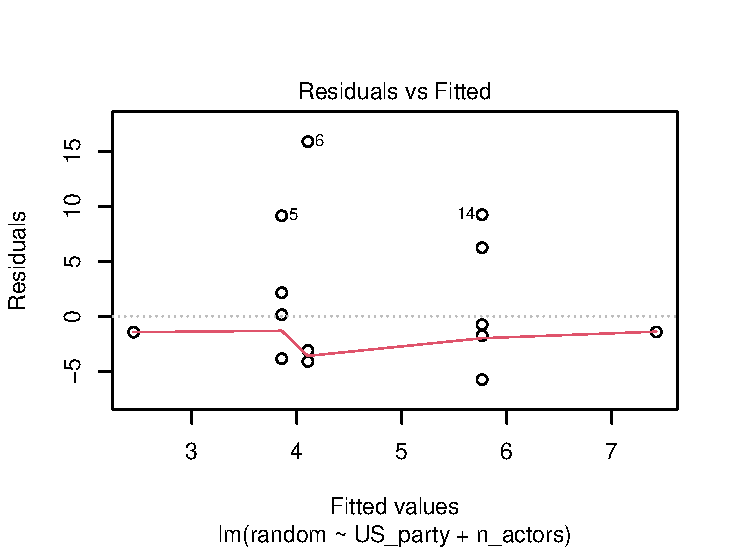
\includegraphics{article_files/figure-latex/lm-1} \end{center}

\end{CodeChunk}

Notice how the regression coefficients change when we pick random values
within the range for the uncertain and approximate dates in the battles
data, in comparison to setting arbitrary cut off points. Although not
statistically significant, the coefficient for US being a party in a
conflict change considerably, going from being positive to becoming
negative, when we we use random values within that range. In this case,
setting arbitrary cut off points to dates introduces a highly
influential outlier observation that affects the model coefficients.
Hence, it is hard to say whether there is a relationship between the US
being an actor involved in one of the battles in 2001 and its duration.

\hypertarget{acknowledgements}{%
\section{Acknowledgements}\label{acknowledgements}}

We would like to thank the Swiss National Science Foundation. This work
was supported by grant number 188976.

\renewcommand\refname{References}
\bibliography{references.bib}



\end{document}
